\documentclass[fleqn,10pt]{SelfArx} % Document font size and equations flushed left

\setlength{\columnsep}{0.55cm} % Distance between the two columns of text
\setlength{\fboxrule}{0.75pt} % Width of the border around the abstract

\definecolor{color1}{RGB}{0,0,90} % Color of the article title and sections
\definecolor{color2}{RGB}{0,20,20} % Color of the boxes behind the abstract and headings

\newlength{\tocsep} 
\setlength\tocsep{1.5pc} % Sets the indentation of the sections in the table of contents
\setcounter{tocdepth}{3} % Show only three levels in the table of contents section: sections, subsections and subsubsections

%----------------------------------------------------------------------------------------
%	ARTICLE INFORMATION
%----------------------------------------------------------------------------------------

\JournalInfo{\ } % Journal information
\Archive{\ } % Additional notes (e.g. copyright, DOI, review/research article)

\PaperTitle{Advanced Computer Architecture: The ``Smooth'' Challenge} % Article title

\Authors{Romain Brault\textsuperscript{1} and Alexandre Camus\textsuperscript{2} and  Giorgos Flourentzos\textsuperscript{3}} % Authors

\affiliation{\textsuperscript{1} \hfill \textsuperscript{2}AC5612 \hfill \textsuperscript{3}}

\Keywords{} % Keywords - if you don't want any simply remove all the text between the curly brackets
\newcommand{\keywordname}{} % Defines the keywords heading name

%----------------------------------------------------------------------------------------
%	USEFULL TOOLS
%----------------------------------------------------------------------------------------

\usepackage[T1]{fontenc}
\usepackage[utf8]{inputenc}

\usepackage[english]{babel}

\usepackage{amsmath}
\usepackage{amsfonts}
\usepackage{amssymb}

\usepackage{enumerate}
\usepackage{caption}
\usepackage{subcaption}
\usepackage{listings}
%\usepackage{hyperref}

% Fonts packages (if needed)
%\usepackage[nott,fullsumlimits]{kpfonts}
%\usepackage{lmodern}

\usepackage{cite}

%----------------------------------------------------------------------------------------
%	ABSTRACT
%----------------------------------------------------------------------------------------

\Abstract{The ABSTRACT is to be in fully-justified italicized text, 
   between two horizontal lines,
   in one-column format, 
   below the author and affiliation information. 
   Use the word ``Abstract'' as the title, in 9-point Times, boldface type, 
   left-aligned to the text, initially capitalized. 
   The abstract is to be in 9-point, single-spaced type.
   The abstract may be up to 3 inches (7.62 cm) long. \\
   Leave one blank line after the abstract, 
   then add the subject categories according to the ACM Classification Index 
   (see http://www.acm.org/class/1998/).}



% ------------------------------------------------------------------------
\begin{document}


%----------------------------------------------------------------------------------------
%	LISTINGS OPTIONS
%----------------------------------------------------------------------------------------

\lstset{
basicstyle=\ttfamily,
keywordstyle=\color{blue},
identifierstyle=,
commentstyle=\color[rgb]{.2,.4,.5},
stringstyle=\ttfamily\color{gray},
breaklines=true}

%----------------------------------------------------------------------------------------

\flushbottom % Makes all text pages the same height

\maketitle % Print the title and abstract box

\tableofcontents % Print the contents section

\thispagestyle{empty} % Removes page numbering from the first page

%-------------------------------------------------------------------------
\section{Introduction}

%% TODO

\subsection{Hardware Considerations}

The chosen hardware is not one of the machine from the Lab. They do not have any interesting GPUs. But one of our laptops is very powerful with an interesting GPU. This is the chosen one.

The table \ref{CPUspec} contains the details of this hardware.
\begin{table}[h]
\centering
\begin{tabular}{|l|r|}
\hline
Model Name & Intel Core i7 CPU Q720 \\
\hline
Clock Speed & 1.597 GHz \\
\hline
Max Turbo Frequency & 2.8 GHz \\
\hline
Cache size & 6144 KB \\
\hline
CPU cores & 4 \\
\hline
CPU Threads & 8 \\
\hline
Integrated GPU & No \\
\hline
Memory Channels & 2 \\
\hline
Max Memory Bandwith & 21 GB/s \\
\hline
\end{tabular}
\caption{CPU Specifications}
\label{CPUspec}
\end{table}

The GPU specifications are shown in the table \ref{GPUspecs}.

\begin{table}[h]
\centering
\begin{tabular}{|l|r|}
\hline
Model Name & NVIDIA GeForce GTX 260M \\
\hline
Clock Speed & 1.375 GHz \\
\hline
Multiprocessors & 14 \\
\hline
Global CUDA cores & 112 \\
\hline
Allocated Memory & 1 GB \\
\hline
Memory Clock Speed & 950 MHz \\
\hline
\end{tabular}
\caption{GPU Specifications}
\label{GPUspecs}
\end{table}

To summarize, the figure \ref{topo} gives a quick overview of the hardware topology. The GPU is connected on the PCI port \verb+10de:0618+.

\begin{figure}[h]
\centering
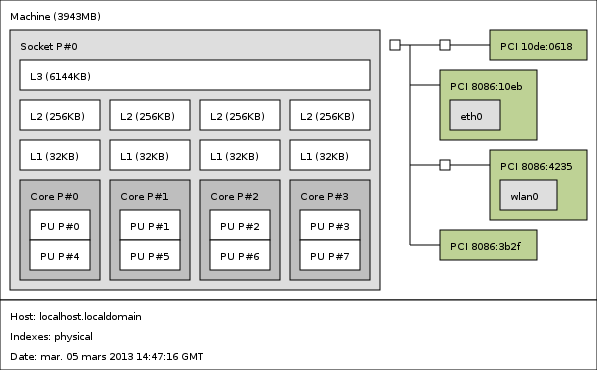
\includegraphics[width=.48\textwidth]{topo.png}
\caption{Topology}
\label{topo}
\end{figure}

\subsection{Software Considerations}

The machine used for this coursework runs a Fedora 18 distribution. This is the exact information:
\begin{lstlisting}
$ uname -a
Linux localhost.localdomain 3.8.1-201.fc18.x86_64 #1 SMP Thu Feb 28 19:23:08 UTC 2013 x86_64 x86_64 x86_64 GNU/Linux
\end{lstlisting}



%-------------------------------------------------------------------------
\section{The Sequential Issue}

After running for the first time the program, it appears that 

Reading the code, some sequential issues were found. There are three kinds of problems: the algorithms chosen, the coding style and the data's representation.

\subsection{Algorithm}

The method used to solve an equations' system was correct but two general to be efficient. The program needs only to solve systems of two equations in two unknowns. The Cramer's rule based on determinants is far more efficient.

The use of the method \verb+pow()+ seems a little too heavy in the method \verb+element_quality()+. As the number of multiplication is known, the use of simple multiplications is more efficient here, e.g. \verb+x*x*x+.

\subsection{Code Style}

Few changes in the style of the code might help the compiler. Some of these changes have been done to speed up the program.

The methods \verb+SVDsolver()+ and \verb+cornerNode()+ and \verb+isSurfaceNode()+ and \verb+element_quality()+ are now written as inline functions. This gives a small boost in performance.

In loops changes have been made to avoid recomputation of the invariant (e.g. in \verb+calling_size()+). Instead, this invariant is now stored in a local variable.

\subsection{Data's Representation}

The data structure used is fine and one of the most efficient to represent a graph. However, the C++ structures used seem to be a little too big in this case. So instead of using vectors of sets, the program is now using vectors of vectors. This increases a little the global performance.

%------------------------------------------------------------------------
\section{CPU Parallelization}

\subsection{Analysis}

Parallelization can't be done easily. The program needs to be slightly modified in order to cut the graph in groups of independent nodes. Independent nodes are nodes that can be inspected at the same time while running the program. To group nodes in such groups the graph must be colored. Then each color represents nodes that can be inspected at the same time because they are not adjacent.

But the coloring algorithm might be very expensive in computation time. This depends on the number of colors used and if this number is specified or not. In this very case, the goal of such an algorithm is to minimize the colors used in order to maximize parallel computations.

\subsection{Optimization}

%-------------------------------------------------------------------------
\section{GPU Acceleration}

\subsection{Analysis}

\subsection{Optimization}

\section{Results}

\subsection{Sequential improvements}

\subsection{GPU performance}

\end{document}